\documentclass[../TDT6.tex]{subfiles}%

\begin{document}
\section{Résolution de problème~: coca-cola}
\QR{%
Par une chaude journée d'été, vous avez oublié de mettre votre soda au frais.
Combien de glaçons faut-il ajouter pour que sa température descende à
\SI{5}{\degreeCelsius}~?
}{%
On pose le système~: transformation isobare donc $\Delta{H} = Q$, et
transformation monotherme. Schéma~:
\begin{center}
	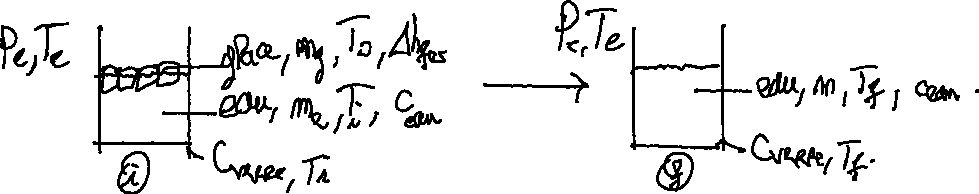
\includegraphics[scale=1]{coca_transfo}
\end{center}
On suppose que le coca est assimilable à de l'eau, de capacité $c\ind{eau} =
	\SI{4.18}{kJ.K^{-1}.kg^{-1}}$. Le système est initialement à l'équilibre, avec
une masse de coca $m_e \approx \SI{250}{g}$ (verre de \SI{300}{mL} pas rempli
à ras bord).
\smallbreak
On suppose que le verre a une capacité thermique non nulle, $C\ind{verre}
	\approx \SI{300}{J.K^{-1}}$ (plus qu'un calorimètre).
\smallbreak
On ajouter une masse $m_g$ de glaçons à $T_0$. Pour connaître leur nombre, il
faut estimer la masse d'un glaçon, sachant que leur densité est $d\ind{glace}
	= \num{0.9}$. En supposant un glaçon cubique de \SI{2}{cm} de côté, on obtient
$m\ind{1glaçon} \approx \SI{7}{g}$.
\smallbreak
On prend $\th_i = \SI{30}{\degreeCelsius}$.
\smallbreak
Reste la plus grosse hypothèse~: adiabatique ou pas~?! On commence par
supposer que oui, soit $\boxed{Q = 0}$. C'est donc un exercice de calorimétrie
classique.
\smallbreak
\noindent
\begin{minipage}[c]{.84\linewidth}
	On suppose un état intermédiaire fictif (possible car $H$ est une fonction
	d'état, donc on peut ajouter et soustraire des transformations) E1 où la glace
	a fondu (à \SI{0}{\degreeCelsius}), et l'eau est à $T_i = \SI{303}{K}$. Sur
	cette transformation,
	\begin{align*}
		\Delta{H}_{\mathrm{eau}, i\to 1}   & = 0 = \Delta{H}_{\mathrm{verre},i\to 1}
		\\
		\Delta{H}_{\mathrm{glace}, i\to 1} & = m_g \Delta{h}\ind{fus}
	\end{align*}
\end{minipage}
\hfill
\begin{minipage}[c]{.15\linewidth}
	\begin{center}
		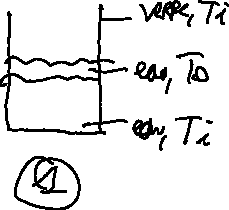
\includegraphics[width=\linewidth]{coca_inter}
	\end{center}
\end{minipage}
Vient ensuite l'autre transformation de $1\to f$, où le verre et l'eau
refroidissent, et la glace maintenant fondue réchauffe~:
\begin{align*}
	\Delta{H}_{\mathrm{eau}, 1\to f}                  & = m_e c\ind{eau} (T_f-T_i)
	\\
	\Delta{H}_{\mathrm{verre},1\to f}                 & = C\ind{verre} (T_f-T_i)
	\\
	\Delta{H}_{\mathrm{glace}, 1\to f}                & m_g c\ind{eau} (T_f-T_0)
	\\\beforetext{Ensuite,}
	\Delta{H}\ind{tot}                                & = \Delta{H}_{i\to 1} + \Delta{H}_{1\to f} = Q = 0
	\\\Lra
	0
	                                                  & =
	m_g \Delta{h}\ind{fus} +
	(T_f-T_i) (m_ec\ind{eau} + C\ind{verre}) +
	(T_f-T_0) (m_gc\ind{eau})
	\\\Lra
	m_g (\Delta{h}\ind{fus} + c\ind{eau} (T_f - T_0)) & =
	(T_i-T_f)(m_ec\ind{eau} + C\ind{verre})
	\\\Lra
	N \cdot m\ind{1glaçon}                            & =
	(T_i - T_f)
	\frac{m_e c\ind{eau} + C\ind{verre}}
	{\Delta{h}\ind{fus} + c\ind{eau}(T_f - T_0)}
	\\\Lra
	\Aboxed{
	N                                                 & =
		\frac{(T_i - T_f)}{m\ind{1glaçon}}
		\frac{m_e c\ind{eau} + C\ind{verre}}
		{\Delta{h}\ind{fus} + c\ind{eau}(T_f - T_0)}
	}
	\\
	\AN
	\makebox[0pt][l]{$\xul{\phantom{N = \num{13.7}}}$}
	N                                                 & = \num{13.7}
\end{align*}
Donc il faudrait un minimum de \SI{14}{glaçons}~! Si on souhaite une
température finale de \SI{8}{\degreeCelsius}, on passe à \SI{12}{glaçons}, ce
qui reste beaucoup.
\bigbreak
Si $Q \neq 0$, alors il faut considérer les pertes thermiques par la surface
du verre et par la surface en contact avec l'air~:
\[
	\left\{
	\begin{array}{llcll}
		\Pc_v        & = g_v S\ind{verre} (T (t) - T_e)
		             & \qav                                 &
		S\ind{verre} & = 2\pi r.h
		\\
		\Pc\ind{air} & = g\ind{air}S\ind{air} (T (t) - T_e)
		             & \qav                                 &
		S\ind{air}   & = \pi r^2
	\end{array}
	\right.
\]
et résoudre une équation différentielle…
}%

\end{document}
